%% LyX 2.3.2-2 created this file.  For more info, see http://www.lyx.org/.
%% Do not edit unless you really know what you are doing.
\documentclass[british]{imaman}
\usepackage[T1]{fontenc}
\usepackage[utf8]{inputenc}
\usepackage{babel}
\usepackage{array}
\usepackage{amsmath}
\usepackage{amsthm}
\usepackage{amssymb}
\usepackage{graphicx}
\usepackage{natbib}
%\usepackage[unicode=true,pdfusetitle,
% bookmarks=true,bookmarksnumbered=false,bookmarksopen=false,
% breaklinks=false,pdfborder={0 0 1},backref=false,colorlinks=false]
% {hyperref}

\usepackage{caption}
\captionsetup[table]{name=\sc Table}
\captionsetup[figure]{name=\sc Fig.}

\input standard.tex

\makeatletter

%%%%%%%%%%%%%%%%%%%%%%%%%%%%%% LyX specific LaTeX commands.
%% Because html converters don't know tabularnewline
\providecommand{\tabularnewline}{\\}

%\addto\captions\british{\renewcommand{\figurename}{Fig.}}
%\addto\captions\british{\renewcommand{\tablename}{tabdd.}}
%\renewcommand\spanishtablename{Otro nombre}

\makeatother

\begin{document}
\title{Tennis Match as Random Walk with Memory: Application to Grand Slam
Matches Modelling}
	\author{
	{\sc Tomáš  Kouřim$^{\dagger}$}\\[2pt]
	Faculty of Nuclear Sciences and Physical Engineering, \\
	Czech Technical University in Prague.\\
	{\rm $^{\dagger}$Corresponding author. Email: tomas.kourim@fjfi.cvut.cz\\[6pt]}
{\sc and}\\[6pt]
	{\sc Petr Volf}\\[2pt]
	Institute of Information Theory and Automation,\\
	Academy of Sciences of the Czech Republic.\\[6pt]
{\rm [Received on 30 November 2019]}\vspace*{6pt}\\
{For Mathsport 2019 special issue.}\vspace*{6pt}
}

\pagestyle{headings}
\markboth{T. KOUŘIM AND P. VOLF}{\rm TENNIS MATCH AS RANDOM WALK WITH MEMORY}
\maketitle
\selectlanguage{british}%
\begin{abstract}
{The contribution introduces a Bernoulli-like random walk with transition
probabilities depending of its recent steps, thus implicitly depending
on the entire walk history. The main objective is its application
to modelling and then to prediction of tennis matches. The model is
applied and tested on men Grand Slam tennis tournaments since
2009. The flexibility of the model is tested thoroughly on several
datasets and the results are presented. It is shown that the model
correctly describes the majority of all matches. Finally, the model
is also used for the in-play real life betting with rather encouraging
results.}

{Random walk, history dependent transition
probability, tennis modelling, prediction, live betting}
\end{abstract}

\section{Introduction}

Tennis is one of the oldest and most traditional sports, which is
pursued worldwide and on all possible levels. It is an industry that
operates with billions of dollars every year. It is therefore no wonder
that even in such a traditional sport as tennis new methods and technologies
are constantly being introduced. Computer imaging is used in the hawk-eye
technology helping to determine whether a ball was out, material science
allows to manufacture better and better rackets and other equipment,
medicine science develops new methods of effective training etc. Mathematics
is becoming a very important part of tennis as well as it can produce
models simulating game situations and predicting their probabilities.
This can be useful for the trainers who can use such models to better
prepare their players for their matches, to detect and prevent frauds,
but most of all it is used for sports betting. The market of sports
betting is despite strict regulations continuously growing both in
revenues as in profits. It is therefore no wonder that the demand
for accurate sports models is tremendous.

There are several different approaches in modelling and simulating
tennis games. The most common ones use Markov chains as the baseline
model, creating Markov-like chains usually from one particular part
of the game --- set by set, game by game, point by point or even rally
by rally (\citealt{barnett2005combining,hunter2009can,newton2009monte,spanias2012predicting}).
Other approaches use some sort of regression --- logistic as in \cite{del2010differences}, or probit as in
\cite{dziedzic2015predicting} or \cite{klaassen2003forecasting}. The methods
can be also divided into those focusing on the match result itself
(\citealt{dziedzic2015predicting,klaassen2003forecasting}), those focusing
on the modelling the match development (the mentioned Markov-like
models), and also concentrated to predict probabilities of partial results during a match ---
\cite{hunter2009can}, this paper (focusing
on the prediction of \emph{in-play }set results). Comparison of some
of the existing methods can be found in \cite{kovalchik2015comparative}.

The final quality of a prediction does not depend on the model used,
but very strongly also on the input information. Such information
can contain data about players (tournament ranking, current form,
past head-to-head results), about the venue (surface, prize money,
ranking points available) and very often also bookmaker's odds, which
is actually sort of an aggregation of all relevant information as shown in \cite{ja2016ddny}.
Bookmaker's odds also serve as an universal benchmark for any prediction
method and models outperforming bookmakers are thus especially interesting.

The present contribution considers the tennis match as a random process,
not insisting on its Markov property. The match in fact consists of
several such processes. A series of sets within a match, games within
a set, points within a game or even strokes within a point can be
all considered a random process and modelled using a random walk.
These walks are well described by the tennis rules and there exist
lots of data describing these random processes (\emph{i.e.} various tennis
result databases provided by the tennis federation as well as many
private subjects). An analysis of non-Markov development in tennis
matches has been provided already in \cite{ja2015ddny}. In the present
paper, the random walk consisting of a sequence of sets within a match
is studied. Matches played as a \emph{best-of-five}, \emph{i.e.} the men
Grand Slam tournaments, are considered. In these matches, up to $5$
steps of the random walk can be observed. The contribution presents
a new version of random walk model with varying transition probabilities
implicitly depending on the history of the walk. The transition probabilities
are altered according to the last step of the walk using a memory
parameter to either reward or punish success by increasing or decreasing
its probability in the next step. It seems more than suitable for
modelling tennis matches as the data suggest that a success in tennis
yields another success, or in other words, that winning one particular
part of the match increases the chances of winning the next part as
well.

The remainder of the paper is organized as follows: First, the model
of Bernoulli-like random walk with transition probabilities dependent
on preceding steps is introduced in Section \ref{sec:Models-of-random}.
Data are described in Section \ref{sec:Data-description}, in Section
\ref{sec:Model-description-and} the model is evaluated and its flexibility
is tested on a historical dataset. The quality of the model is assessed
also via its use in real life betting and the results are described
in Section \ref{sec:Test-by-betting}. Finally, Section \ref{sec:Conclusion}
concludes this paper.

\section{Models of random walk with memory\label{sec:Models-of-random}}

A basic type of a discrete time random walk is the Bernoulli walk,
with random steps (denote them $X_{i}$ at stage $i$) $X_{i}=\pm1$,
with constant transition probability $P(X_{i}=1)=p_{0}$. It is a
representation of a Markov chain, \emph{i.e.} a memory-less random process.
It may fit perfectly to many real processes, however, many others,
including the tennis match development, are more complex, and a memory
element has to be introduced in order to correctly describe them.
Then $p_{0}$ can be regarded as an input parameter based on initial
match conditions, and the transition probabilities evolve depending
on the match progress.

Naturally, the idea of process transitions depending on the history
of process itself is not new. An inspiration can be found for instance
in the statistical modelling of recurrent events in lifetime (reliability)
analysis. For the case analysed in the present paper, with discrete
time and only several steps in a walk, the regression model is not
considered (though the use of logistic regression is a natural generalization
here) and the transition probabilities are changed just by multiplying
them by a convenient parameter. An inspiration to such a modification
of Bernoulli random walk can be found in several papers where the
length of step was changed in a similar way. \cite{turban2010random} presented
a model of a one-dimensional random walk with memory introduced through
varying step size. In the paper, it is
assumed that the step size in the direction of the last step will
be lowered by a coefficient $\lambda$ and the step in the opposite
direction will be prolonged so that the sum of absolute values of
the steps remains constant and equal to $2$. The goal is to stabilize
the process. Another interesting variant of model is presented in \cite{schutz2004elephants} introducing a special
type of a random walk with the random increment at time step $t$
depending on the full history of the process (compared to an elephant's
memory in the paper). The walk tends to repeat `good decisions'
(\emph{i.e.} steps from history). The present application keeps constant
steps length but instead changes the transition probabilities.

\subsection{Transition probabilities dependent on process history}

The concept of the model has been introduced by \cite{ja2017ddny}.
It is based on the standard random walk with steps $X_{i}=\pm1,\,i=1,2,...$.
The distribution of the first random variable $X_{1}$ is given by
a starting parameter $p_{0}\in[0,\,1]$, so that $P(X_{1}=1)=p_{0}$
and $P(X_{1}=-1)=1-p_{0}$. After the $i$-th step (for $i\ge1$),
the probability distribution of the next step $X_{i+1}$ is given
by the (random) probability $p_{i}$, which depends on a coefficient
$\lambda\in[0,\,1]$ and the last random variable $X_{i},\,i=1,2,...$:
\[
p_{i}=\lambda p_{i-1}\,\,\mbox{for}\,\,X_{i}=1,
\]
\[
p_{i}=1-\lambda(1-p_{i-1})\,\,\mbox{for}\,\,X_{i}=-1,
\]
which yields that 
\begin{equation}
p_{i}=\lambda p_{i-1}+\frac{1}{2}(1-\lambda)(1-X_{i}).\label{eq:pi-punish}
\end{equation}
The case with $\lambda=1$ corresponds to the standard Markov random
walk with constant transition probability, with $\lambda=0$ the walk
would be a series of alternating steps to the left and right with
only the first step direction being chosen randomly. Therefore only
$\lambda\in(0,\,1)$ is further considered. As after each `success'
($X_{i}=1$) the probability of its repetition in the next step decreases,
we can call this scheme a `success punished' model. Naturally, the
opposite, a `success rewarded' variant, is possible, which leads
to a similar expression for $\bar{p}_{i}=1-p_{i}$: 
\begin{equation}
\bar{p}_{i}=\lambda\bar{p}_{i-1}+\frac{1}{2}(1-\lambda)(1-X_{i})\label{eq:pi-reward}
\end{equation}
for $i=1,2,...$.

Another alternative is a random walk with each event influencing the
further development of the walk differently, which can be expressed
as
\begin{equation}
p_{i}=\frac{1}{2}[(1+X_{i})\lambda_{0}p_{i-1}+(1-X_{i})(1-\lambda_{1}(1-p_{i-1}))],\label{eq:pi-2lambda}
\end{equation}
with $\lambda_{0},\,\lambda_{1}\in(0,\,1)$, or a similar model for
parameters $\bar{p}_{i}=1-p_{i}$. Other alternatives of the model
can be considered as well. For example, parameter $\lambda$ can depend
on available covariates in a logistic manner, the transition probabilities
can depend explicitly not only on the last step, but on longer history
or also on the number of steps, the walk can be defined in a multidimensional
space or on a graph, and other generalizations.

The behaviour of the proposed random walk types was analysed in \cite{ja2017ddny},
focusing on the development after a large number of steps (\emph{i.e.} asymptotic
properties). In the present application the walk consists of just
a small number of steps, the long-run properties overview is thus
omitted here. The main task of this paper is therefore assessing the
initial probability $p_{0}$ and reliable estimation of parameters
$\lambda$. Another task is to recognize which type of model is the
most convenient. In the following real data analysis the `success
rewarded' model variant was selected, after a thorough data analysis
proved that tennis match develops according to this model type as shown in \cite{ja2014ddny}.

\section{Data description\label{sec:Data-description}}

Two datasets were acquired for the purpose of this paper, one for
model development and the other for model testing. The development
dataset contains the results from all Grand Slam tournaments from
2009 to 2018 and corresponding Pinnacle Sports bookmaker's odds (Pinnacle
Sports bookmaker was chosen as it is considered leading in the sports
betting industry). It was created using data publicly available from
website www.oddsportal.com. Every year 4 Grand Slam tournaments (\emph{i.e.}
Australian Open, French Open, The Wimbledon and US Open) are played,
making it $40$ tournaments during the selected period. Each Grand
Slam has $128$ participants in the men singles category played in
a single-elimination system (\emph{i.e.} $127$ games per tournament). Thus,
there were $5080$ matches available altogether. Some matches were
not finished due to one of the players forfeiting and such matches
were omitted from the dataset. Matches without bookmaker's odds were
omitted as well. The final dataset contains $4255$ matches with complete
data available, played by $432$ players in total. The most active
player was Novak Djokovic, who participated in $188$ matches. On
average, each player played $19.7$ matches, with the median value
of $8$ matches played. The most common result was 3:0, occurring
$2138$ times, on the other hand, 5 sets were played only $808$ times.

The order in which the players are listed is rather random. The players
listed first won $2201$ in total, just slightly over the half. The
player listed first would be normally considered as `home', however,
as there are (usually) no home players on the international tournaments,
the order is based on the www.oddsportal.com data and/or the respective
tournament committees. On the other hand, if the bookmaker's favourite
(\emph{i.e.} the player with better odds or the first listed player in case
the odds are even) is considered, the situation changes significantly.
The favourites won $3307$ matches in total, mostly 3:0, and lost
$311$ times 0:3, $347$ times 1:3 and $290$ times 2:3. It suggests
that bookmaker's odds can be used as a winning probability estimate,
which is in accordance with previous results, for example in \cite{ja2016ddny}.

Evaluation dataset was created in order to further validate the quality
of the presented model. It consists of the 2019 men singles US Open
matches, with the results and set winning odds provided by Tipsport
(the biggest Czech bookmaker). The major difference between the two
datasets is the fact that the evaluation dataset contains not only
\emph{pre-match} odds, but\emph{ in-play} odds as well, and can be
thus used to evaluate the model quality in real life setting. There
were $127$ matches and $448$ sets played in total during 2019 men
tennis US Open, the created dataset contains $423$ set odds ($25$
set odds missing due to website malfunction, not being provided by
the bookmaker or some other problems).

\section{Application of random walk\label{sec:Model-description-and}}

Original inspiration of the random walk described in Section \ref{sec:Models-of-random}
is based on intensive study of historical sport results and their
development. The data suggest that the probability of success (\emph{i.e.}
scoring, winning a set or a point etc.) evolves according to the random
walk with varying probabilities. Moreover, it follows from the data
that sports can be very roughly divided into two categories. Sports
played for a certain amount of time, such as soccer or ice-hockey,
evolve according to the walk defined by expression (\ref{eq:pi-punish}).
On the other hand, sports where there is necessary to achieve certain
number of points, such as tennis or volleyball, appear to follow the
pattern defined in equation (\ref{eq:pi-reward}). Therefore the later
approach is used to model a tennis game.

The model is used to predict the winning probabilities of sets $2$
through $5$ and is constructed in a following manner. For each match,
the first set winning probability of Player A (the player which is
listed first in the database), $p_{0}$, is given by an initial probability
and a coefficient $\lambda$ is fixed for the entire dataset. In order
to compute the second set winning probability, the result of the first
set is observed and second set winning probability is computed using
equation (\ref{eq:pi-reward}). This procedure is repeated for all
remaining sets played (there can be either $3$, $4$ or $5$ sets
played in total in a \emph{best-of-five} tennis game).

\subsection{Initial probability derivation\label{sec:Initial-probability-derivation}}

The model (\ref{eq:pi-punish}) or (\ref{eq:pi-reward}) of a random
walk with varying probabilities described in Section \ref{sec:Models-of-random}
contains two parameters, initial set winning probability $p_{0}$
and the memory coefficient $\lambda$. Finding the optimal value of
$\lambda$ is described further. Estimating the initial set winning
probability is a major task by itself and represents one of the elementary
problems in tennis modelling (and sports predictions in general).
For the purpose of this article an estimation based on bookmaker's
odds will be used. Specifically, the closing odds (closing odds means
the last odds available before the match started) by Pinnacle Sports
bookmaker for the first set result are used to estimate the probabilities
of each player winning the first set. Such odds represent a good estimation
of the underlying winning probability and are considered as a baseline
in the sports betting industry. The odds, however, have to be transformed
into probabilities. A method described in \cite{ja2015ddny} is used
to obtain probabilities, which in case of only two possible outcomes
(such as in tennis match) can be expressed as 
\[
p_{i}=\frac{1}{a_{i}}-(G-1)[1-\frac{1}{a_{i}G}+2\omega(\frac{1}{a_{i}G}-0.5)],\;i\in\{1,\,2\},
\]
where $p_{i}$ are the unknown first set winning probabilities, $a_{i}$
the corresponding odds provided by bookmaker and $G=\sum_{i=1}^{2}\frac{1}{a_{i}}$.
A parameter $\omega\in[0,\,1]$ is used to spread bookmaker's margin
among the two outcomes and for the purpose of this paper it is set
to the value $\omega=0.5$. Obtained first set winning probabilities
are then used as a given starting probability $p_{0}$ in the random
walk.

\subsection{\label{subsec:Model-evaluation}Model evaluation}

In order to verify the model accuracy, several tests were performed.
First, the dataset was divided into training and testing sets. The
division can be done naturally by the order of games played. Given
a specific time, past matches constitute to a training set, future
matches to a testing set. For the purpose of this paper, the split
was done on a yearly basis, the data from one previous tennis season
were used as a training set to predict winning probabilities in the
following season, considered the testing set (\emph{i.e.} 2010 was the first
season used as testing data, 2017 was the last season used as training
data), making it 9 training/testing splits together. Another approach
to dataset splitting is to consider data from all previous years as
testing data and from one future year as training data, however, previous
study by \cite{ja2016ddny} shows that the difference between these two approaches is negligible.

Next step in model evaluation is the estimation of parameter $\lambda$.
Training sets and maximal-likelihood estimates (MLE) were used for
this task. The likelihood function is defined as 
\[
L=\prod_{i=1}^{N_{train}}(x_{i}p_{i}+(1-x_{i})(1-p_{i})),
\]
where $N_{train}$ is the number of sets $2$ through $5$ played
in the training dataset, $p_{i}$ is Player A's winning probability
in the $i-th$ set obtained using the method described above for each
match, and $x_{i}$ is the result of the $i-th$ set, $x_{i}=1$ if
Player A won the $i-th$ set, $x_{i}=0$ otherwise. For computational
reasons the \emph{log-likelihood }$L_{l}=log(L)$ was used, \emph{i.e.} the
function 
\[
L_{l}=\sum_{i=1}^{N_{train}}log(x_{i}p_{i}+(1-x_{i})(1-p_{i}))
\]
was maximized. Numerical methods implemented in Python library SciPy
were used to obtain specific values of $\lambda$. The optimal values
of the coefficient $\lambda$ can be seen in Table \ref{tab:Optimal-values-of}.

\begin{table}
\begin{centering}
\begin{tabular}{|c|c|}
\hline 
Year & Optimal lambda\tabularnewline
\hline 
\hline 
2010 & 0.8074\tabularnewline
\hline 
2011 & 0.8497\tabularnewline
\hline 
2012 & 0.8142\tabularnewline
\hline 
2013 & 0.9162\tabularnewline
\hline 
2014 & 0.8523\tabularnewline
\hline 
2015 & 0.8429\tabularnewline
\hline 
2016 & 0.8920\tabularnewline
\hline 
2017 & 0.8674\tabularnewline
\hline 
2018 & 0.8333\tabularnewline
\hline 
\end{tabular}
\par\end{centering}
\caption{\label{tab:Optimal-values-of}Optimal values of the coefficient $\lambda$
for respective years}
\end{table}

Finally, the model was used to predict set winning probabilities of
the unseen data from the training set using initial bookmaker derived
odds, equation (\ref{eq:pi-reward}) and memory parameter $\lambda$
obtained from the corresponding training set. In order to verify the
quality of the model, the average theoretical set winning probability
of Player A $\hat{p}=\frac{1}{n}\sum_{i=1}^{N_{test}}p_{i}$ and its
variance $\hat{\sigma}^{2}=\frac{1}{n}\sum_{i=1}^{N_{test}}p_{i}(1-p_{i})$
were computed and so was the observed Player A winning ratio $\bar{x}=\frac{1}{n}\sum_{i=1}^{N_{test}}x_{i}$.
Using the Lyapunov variant of Central Limit Theorem (CLT), the resulting
random variable $y$ follows the standard normal distribution 
\begin{equation}
y=\frac{\sqrt{N_{test}}(\bar{x}-\hat{p})}{\hat{\sigma}}\thicksim\mathcal{N}(0,\,1).\label{eq:CLT}
\end{equation}
Then in order to verify the model accuracy, the null hypothesis that
the true average Player A set winning probability $\bar{p}$ equals
$\hat{p}$ against the alternative hypothesis $\bar{p}\neq\hat{p}$
was tested. Formally, $H_{0}:\bar{p}=\hat{p}$, $H_{1}:\bar{p}\neq\hat{p}.$

One of the assumptions of the CLT is that the observed random variables
are independent. This is obviously not true in the case when $N_{test}$
contains all sets from the testing data. Quite the opposite, the model
assumes that the winning probability of a set directly depends on
the winning probability of the previous set. This can be easily solved
by splitting the testing dataset into $4$ subsets containing only
results from single set of each match, \emph{i.e.} sets $2$, $3$, $4$
and $5$ (if they were played). The matches can be considered independent
from each other and so can be the $i-th$ sets of respective matches.

Using this approach, there are $36$ testing data subsets together
(up to $4$ sets considered in each match, $9$ yearly testing datasets).
On a $95\%$ confidence level, only on $2$ out of the $36$ available
subsets provide strong enough evidence to reject the null hypothesis.
On the other hand, the null hypothesis is relatively weak. It only
says that the prediction is correct on average. In order to verify
the quality of the predictions, more detailed tests have to be created.
This can be done primarily by testing the null hypothesis on many
subsets created according to some real life based criteria. The natural
way how to create such subsets is dividing the matches to the $4$
different tournaments. This refining yields $180$ subsets: $4$ sets
in each match evaluated, $4+1$ tournaments every year, $9$ years
for testing. Using $95\%$ confidence level, only $6$ of the $180$ subsets have data strong
enough to reject the null hypothesis. It is worth mentioning that
the size of some of the datasets regarding fifth sets is only slightly
above $20$ observations, which can interfere with the assumptions
justifying the use of CLT.

To further analyse the robustness of the model it is important to
realize the structure of the data. So far, the player, whose winning
probability was estimated, was chosen arbitrarily based on some external
(more or less random) order. As such, the observed winning probability
in every subset equals approximately to $\frac{1}{2}$. In such a
dataset it is not very difficult to estimate the average winning probability.
The situation changes if the bookmaker's favourite is considered for
predictions. Performing the same tests as described in the previous
paragraph the data allows to reject the null hypothesis (on a $95\%$
confidence level) on $5$ subsets containing all tournaments and $8$
single tournament subsets (out of $180$ subsets total).
\begin{figure}
\centering{}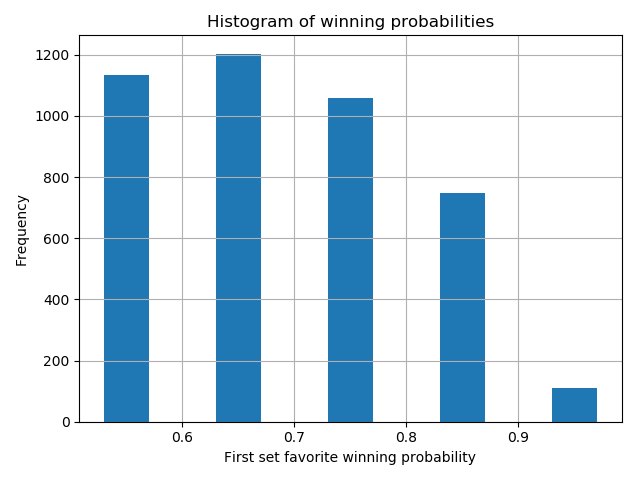
\includegraphics[width=0.8\textwidth]{../conference_paper/probabilities_histogram}\caption{\label{fig:First-set-winning}First set winning probability $p_{0}$
histogram.}
\end{figure}

Finally, the testing data can be divided into groups using the initial
probability $p_{0}$. Such a division is based on an assumption that
the matches with similar bookmaker odds should have similar development.
The matches are divided into $5$ groups, each containing $10$ percentage
points in first set winning probability. Except for the biggest favourites
(with first set winning probability over $90\%$), this division seems
reasonable. The data histogram can be seen on Fig. \ref{fig:First-set-winning}.
Out of the $180$ newly created odds-based subgroups, only $9$ have
data strong enough to reject $H_{0}$ on a $95\%$ confidence level.
The entire results of the hypothesis testing (the \emph{p-values }of
respective tests) can be seen on Fig. \ref{fig:p-values-of-hypothesis}.
More detailed division, \emph{i.e.} by tournament and odds, was not performed
as the resulting datasets would not contain enough data.

Overall, the model was tested on $360$ different subsets and only
$22$ of them ($6.1\%$) provided enough evidence to reject $H_{0}$
on $95\%$ confidence level. These subsets are distributed randomly
and there is no pattern among them, indicating there is no systematic
bias in the model. The random walk with varying probabilities thus
seems to be a robust model which can be used to precisely predict
set winning probabilities in men tennis Grand Slam matches.
\begin{figure}
\centering{}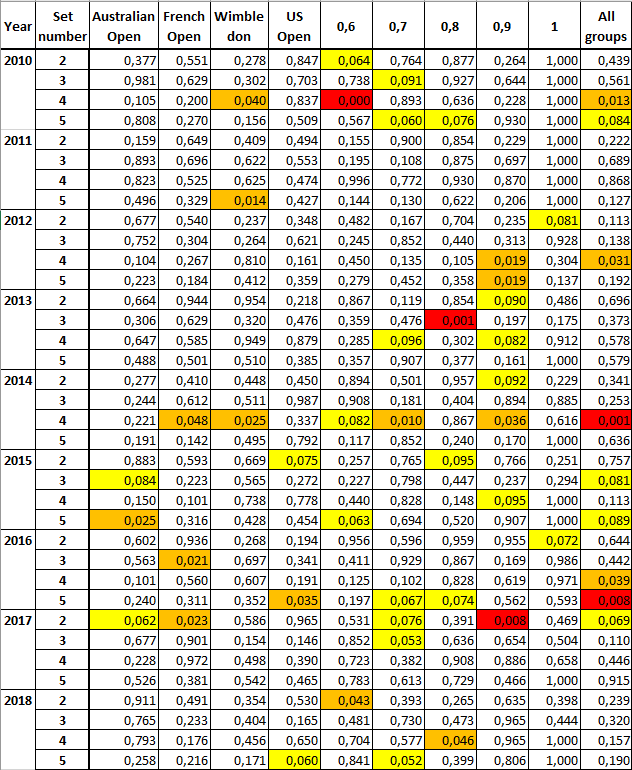
\includegraphics[width=1\textwidth]{../conference_paper/hypothesis_testing.PNG}\caption{\emph{\label{fig:p-values-of-hypothesis}p-values} of hypothesis tests
for different testing sets. Red are marked those allowing to reject
$H_{0}$ on 99\% confidence level, orange on 95\% and yellow on 90\%
confidence level (or dark, grey and pale highlighting respectively for grayscale print).}
\end{figure}

\section{Model testing\label{sec:Test-by-betting}}

The model was implemented and tested in real life setup where it actively
bet \emph{ in-play} against Tipsport, the biggest bookmaker in the Czech Republic.
The test was set up in the following manner.

An automated betting and odds scraping tool developed using the Python
programming language and Selenium framework running on a remote server
(Digital Ocean) was developed and deployed for the purpose of this
paper. The tool operates with Tipsport's website and scrapes it for
both \emph{pre-match }as well as \emph{in-play} odds. It was set up
to continuously observe Tipsport's odds offerings for 2019 men tennis
US Open, especially the set winning odds, and store the odds together
with some general information about the match, such as the respective
players, starting time etc., into a database (Postgresql database).
To test the model, Tipsport's starting odds were used to obtain parameter
$p_{0}$ (as described above) and (according to the results from Section
\ref{sec:Model-description-and}) optimized $\lambda$ trained on
the $2018$ tennis season was chosen as the second necessary model
parameter. Every match was observed individually and after each finished
set next set winning probabilities were computed using the presented
model. Whenever the actual set winning odds offered by Tipsport for
one of the players $a_{i}$ were higher than the probability implied
set winning odds for that player computed by the model, \emph{i.e.} $a_{i}>\frac{1}{p_{i}}$,
a bet was made. The amount bet was computed as $p_{i}U$, where $U$
is a base bankroll-dependent betting unit. This amount was further
rounded with precision CZK $1$ (due to betting limitations of Tipsport).
Overall, $128$ bets were made (and $3$ additional bets that were
cancelled due to one of the players forfeiting the match because of
injury) with the total amount $59.85U$ bet. The expected number of
wins among these bets was $59.85$ whereas the actual number of wins
was $57$. Using the same hypotheses testing as in Section \ref{subsec:Model-evaluation},
the data showed no evidence to reject $H_{0}$ ($p$-value $\sim0.59$).
The minimal account balance over the entire US Open was $-0.52U$
and the final balance $2.24U$, creating a theoretical return on investment
(ROI) of $430\%$ within only 2 weeks, which is an outstanding performance.

\subsection{Alternative betting strategies}

Choosing the correct betting strategy is one of the key elements of
successful betting. It depends on the underlying model, available
bookmaker's odds, bankroll, internal bookmaker's policies and many
other parameters. There exists a large number of possible approaches
and the detailed description of them is beyond the scope of this paper.
Besides the implemented strategy, where an amount proportional to
$p$ was bet on each selected opportunity, two other basic betting
strategies were applied to test the model. A strategy where always
$\frac{1}{a}$, \emph{i.e.} the inverse value of odds, was bet, and a naive
strategy with simply $1$ unit put on every bet. 

The strategies differ in the expected wins and their variance. The theoretical properties
of the betting strategies can be observed in Table \ref{tab:strategies}
with the special case where $p=\frac{1}{a}$, \emph{i.e.} in case of fair
odds (see \citealt{ja2015ddny}). The results of the different betting strategies
applied together with the presented model to bet on 2019 men US Open
(actual for probability based strategy and theoretical for other strategies)
are shown in Table \ref{tab:The-results-of}. The development of the
account balance for different betting strategies is displayed on Fig.
\ref{fig:Account-balance-development}. The figure shows that the
general shape of balance development is very similar for all three
strategies. This is caused by the fact that all strategies bet on
the same opportunities, \emph{i.e.} only when the expected win from the bookmaker's
odds is positive according to the presented model ($a_{i}>\frac{1}{p_{i}}$
holds for some offered betting opportunity), and only differ in the
amount bet. The naive strategy then reaches the most extreme values,
which is caused by its variance, the biggest among selected variants
(as shown in Table \ref{tab:strategies}).

\begin{table}
\begin{centering}
\begin{tabular}{|c|c|c|c|c|c|}
\hline 
Strategy & Bet & $E(w)$ & $E(w|p=\frac{1}{a})$ & $Var(w)$ & $Var(w|p=\frac{1}{a})$\tabularnewline
\hline 
\hline 
Naive & $1$ & $pa-1$ & $0$ & $pa^{2}(1-p)$ & $a(1-\frac{1}{a}$)\tabularnewline
\hline 
Odds & $\frac{1}{a}$ & $p-\frac{1}{a}$ & $0$ & $p(1-p)$ & $\frac{1-\frac{1}{k}}{k}$\tabularnewline
\hline 
Prob. & $p$ & $p(pa-1)$ & $0$ & $p^{3}a^{2}(1-p)$ & $\frac{1-\frac{1}{k}}{k}$\tabularnewline
\hline 
General & $u$ & $u(pa-1)$ & $0$ & $u^{2}pa^{2}(1-p)$ & $u^{2}a(1-\frac{1}{a})$\tabularnewline
\hline 
\end{tabular}
\par\end{centering}
\caption{\label{tab:strategies}Theoretical values of wins and variances for
different betting strategies}

\end{table}

\begin{table}
\begin{centering}
\begin{tabular}{|c|>{\centering}p{1.5cm}|>{\centering}p{1.5cm}|>{\centering}p{1.5cm}|c|c|}
\hline 
Strategy & Expected profit & Profit std. dev. & Minimal balance & Profit & ROI\tabularnewline
\hline 
\hline 
Naive & $11.1$ & $15.17$ & $-3.62$ & $2.99$ & $83\%$\tabularnewline
\hline 
Odds & $4.07$ & $5.29$ & $-0.72$ & $1.23$ & $171\%$\tabularnewline
\hline 
Prob. & $4.91$ & $5.79$ & $-0.52$ & $2.24$ & $430\%$\tabularnewline
\hline 
\end{tabular}
\par\end{centering}
\caption{\label{tab:The-results-of}The results of different betting strategies
applied to US Open betting using the presented model}
\end{table}


\begin{figure}
\begin{centering}
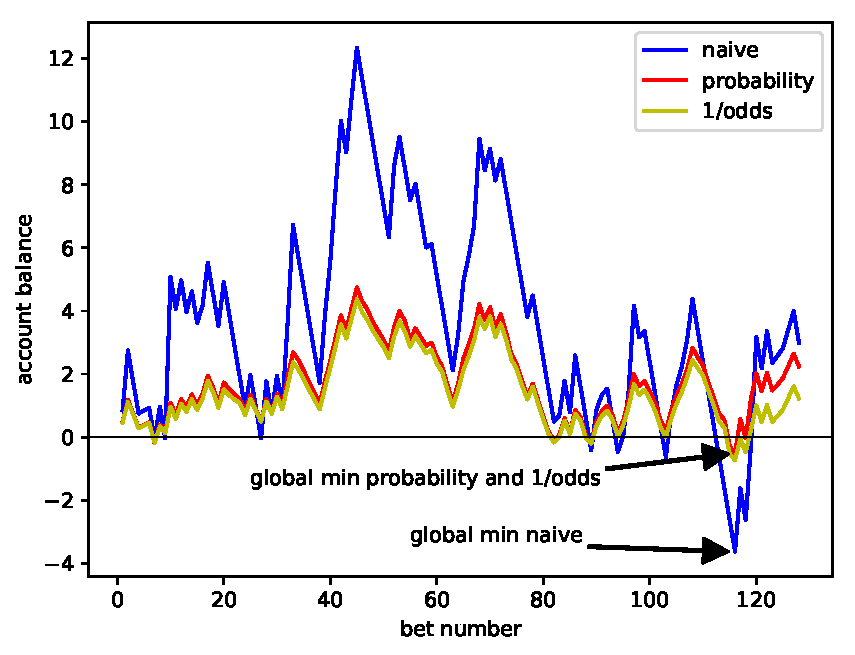
\includegraphics[width=0.8\textwidth]{../../betting_analysis/account_balance_development}

\caption{\label{fig:Account-balance-development}Account balance development
for different betting strategies.}
\end{centering}
\end{figure}



\section{Concluding remarks\label{sec:Conclusion}}

In the present paper, a model of Bernoulli-like random walk with transitions
dependent on the walk history was introduced. A number of variations
of this model was described by the authors in a recent study \cite{ja2019apmat}.
This paper shows that even the rather simple version presented here
shows sufficient flexibility and can be applied to tennis matches
modelling. The model was first tested statistically on historical
data and the optimal model parameters were computed using numerical
methods. The results were then tested in real \emph{in-play }betting
against a commercial bookmaker with rather encouraging results. This
show a huge potential of the model being able to describe even the
most complicated real life discrete random processes with memory.
The application of the model on different real life problems will
be subject of further research.

The source code containing all functionality mentioned in this article
including the automated betting engine is freely available as open
source at GitHub (https://github.com/tomaskourim/mathsport2019) together
with a database containing data used in this paper. Some
more results can be also obtained from the same repository.

\section*{Funding}

This work was supported by the Grant
Agency of the Czech Republic [18-02739S].

\bibliographystyle{IMANUM-BIB}
\bibliography{../conference_paper/doktknih}

\end{document}
